\documentclass[conference]{IEEEtran}
\usepackage{cite}
\usepackage{amsmath,amssymb}
\usepackage{booktabs}
\usepackage{graphicx}
\usepackage{url}
\usepackage{array}
\usepackage{xcolor}
\usepackage{tikz}
\usepackage{pgfplots}
\usepackage{algorithmic}
\usepackage{balance}
\usetikzlibrary{arrows.meta,positioning}
\pgfplotsset{compat=1.18}
\definecolor{baseline}{HTML}{65758B}
\definecolor{language}{HTML}{DC9439}
\definecolor{proposed}{HTML}{087F8C}
\definecolor{heatlow}{HTML}{FFFFDA}
\pgfplotsset{paperaxis/.style={
    font=\footnotesize, tick label style={font=\scriptsize},
    label style={font=\footnotesize}, axis lines*=left,
    ymajorgrids, grid style={black!12}, tick align=outside}}
\newcommand{\ind}{\mathbf{1}}
\title{Physics-Constrained AI Agents for Automated Quantum Circuit Debugging and Repair}
\author{\IEEEauthorblockN{Alok Pandey}\IEEEauthorblockA{Indian Institute of Technology Patna}}
\begin{document}
\maketitle

\begin{abstract}
Quantum-circuit debugging is difficult because a syntactically valid or logically plausible repair may still violate hardware-native gates, connectivity, or noise-aware execution requirements. This paper presents a physics-constrained agentic framework that couples fault localization and minimal candidate generation with compilation and explicit validation. A structured circuit state records diagnostics and repair history; failed checks provide feedback for subsequent attempts. The reported benchmark comprises 1,000 buggy circuits, five bug classes, and three compared systems. The proposed agent achieves Pass@1 of 77.5\%, Pass@3 of 99.1\%, and physics validity of 99.2\%, with 1.31 mean repair iterations. Architecture and circuit diagrams explain the workflow, while comparative plots expose success rates, category coverage, and structural overhead. The evaluation uses the IBM FakeSherbrooke hardware model rather than live-device execution. The reported improvements are interpreted alongside unequal retry use, incomplete configuration records, and the limits of aggregate statistics. These results motivate validation-centered quantum repair, without establishing that every gain is attributable to physical constraints alone.
\end{abstract}
\begin{IEEEkeywords}
quantum software engineering, circuit debugging, AI agents, automated program repair, hardware-aware compilation
\end{IEEEkeywords}

\section{Introduction}
Quantum programs require agreement between a high-level computational specification and a physically executable circuit. A local code edit can resolve a parser error while introducing a wrong qubit operand, changing an entangling operation, or generating a gate sequence that is unsuitable for the target device. Conversely, a correct abstract circuit can need additional decomposition and routing before it can be executed. These distinctions make repair more demanding than producing code that merely looks plausible.

Language-model-assisted quantum repair has been explored through direct patch generation and simulation-based debugging pipelines \cite{guo2024repairing,pham2026qbuglm}. Symbolic circuit simplification and learning-based optimization offer complementary ways to transform circuits \cite{duncan2020graph,quarl2024}. However, an optimization that preserves the behavior of a buggy program does not necessarily restore the intended computation. Likewise, a generated repair is not evidence of correctness until an independent oracle evaluates its behavior and target compatibility.

We study the question: \emph{Can a physics-constrained AI agent improve semantic repair and hardware-model validity compared with symbolic and language-model baselines?} The proposed architecture makes validation part of the decision loop. The agent localizes a suspected fault, proposes a limited edit, compiles the candidate, and receives structured results from semantic and physical checks. Acceptance requires successful checks rather than a high language-model confidence score.

The contributions are threefold. First, we specify a repair architecture with explicit state, a hard acceptance predicate, and diagnostic feedback. Second, we organize the reported 1,000-circuit comparison using success, physics validity, iteration cost, and structural overhead. Third, we analyze what these aggregate results support and which claims require additional evidence. All numerical plots use the supplied benchmark summaries; the circuit illustration is explanatory rather than an additional measured experiment.

\section{Related Work and Scope}
\subsection{Language-Guided Quantum Repair}
Guo \emph{et al.} investigate the use of ChatGPT to repair quantum programs, establishing a direct connection between language-model generation and quantum software maintenance \cite{guo2024repairing}. QBugLM provides an agentic benchmarking framework covering bug injection, detection, repair, and simulation-based validation \cite{pham2026qbuglm}. Importantly, QBugLM itself includes iterative feedback. Therefore, the single-attempt QBugLM row in the present comparison describes the supplied evaluation configuration, not a general inability of that framework to retry or use tools.

The proposed distinction is consequently not simply that an agent uses feedback. It is that target-model compatibility and physical checks are explicit acceptance requirements alongside semantic correctness. A fair assessment of that distinction needs matched language models, comparable tool access, and equal retry budgets. Those controls are not fully documented in the available aggregate record, so the evaluation should be read as a comparison of reported system configurations.

\subsection{Symbolic and Learning-Based Transformation}
ZX-calculus simplification transforms circuits through a graph representation and can preserve their represented computation while reducing structure \cite{duncan2020graph}. This makes PyZX a useful symbolic transformation baseline, but not a direct replacement for repair guided by a specification. If a circuit implements the wrong computation, equivalence-preserving simplification alone need not fix it. Quarl instead learns a policy for selecting circuit transformations from a large optimization space \cite{quarl2024}. Such techniques can support candidate optimization, while correctness must still be defined relative to the intended task.

\subsection{Physical Constraints and Execution Models}
Physics-constrained learning also appears at the quantum-control level, where allowable signal dynamics and realistic control restrictions shape the search space \cite{ernst2025physical}. Our framework operates at the circuit-repair level rather than claiming pulse-level control. Its hardware checks use FakeSherbrooke and a model-based execution setting. IBM describes backend-derived noise models as approximations of device errors \cite{ibmnoise}; passing those checks is therefore distinct from demonstrating fidelity on a live quantum processor.

\section{Problem Formulation}
Let $C_{\mathrm{bug}}$ be a buggy circuit, $\mathcal{O}$ an oracle describing intended behavior, and $\mathcal{B}$ a target hardware model. A repair procedure seeks a candidate $C^\star$ that satisfies the specification and remains acceptable after compilation. The oracle must come from a trusted reference circuit, a task specification, or independent tests; it must not be silently replaced by the behavior of the buggy input.

Write $\widetilde C=T_{\mathcal B}(C)$ for the compiled candidate. We separate four validation predicates:
\begin{equation}
\begin{split}
 A(C;\mathcal O,\mathcal B)={}&V_{\mathrm{syn}}(C)\land V_{\mathrm{str}}(C)\\
 &\land V_{\mathrm{sem}}(\widetilde C,\mathcal O)
 \land V_{\mathrm{phys}}(\widetilde C,\mathcal B).
\end{split}
\label{eq:accept}
\end{equation}
Compilation failure makes acceptance false. Syntax and structure concern legal instructions and operand use; semantics concerns the intended computation; physical validity concerns the selected target and model-based execution requirements. These predicates need not be statistically independent.

\begin{table}[t]
\caption{Bug taxonomy and illustrative validation evidence. Each category contains 200 reported instances. Examples specify the intended checking role, not additional measured cases.}
\label{tab:taxonomy}
\centering\footnotesize
\setlength{\tabcolsep}{4pt}
\begin{tabular}{@{}>{\raggedright\arraybackslash}p{0.20\columnwidth}>{\raggedright\arraybackslash}p{0.34\columnwidth}>{\raggedright\arraybackslash}p{0.37\columnwidth}@{}}
\toprule
Category & Illustrative fault & Relevant evidence\\
\midrule
Physics & Target-incompatible interaction & Compilation and target checks\\
Structural & Invalid qubit index or arity & Register and operand checks\\
Semantic & Incorrect gate or parameter & Independent behavior oracle\\
Syntax & Malformed instruction & Parser diagnostics\\
Redundancy & Unnecessary gate pair & Equivalence and resource counts\\
\bottomrule
\end{tabular}
\end{table}

The taxonomy in Table~\ref{tab:taxonomy} separates failures that need different evidence. A syntax fix can be judged locally, whereas changing a rotation angle may require a behavior-level comparison. A redundant inverse pair can preserve ideal semantics yet increase execution cost. Thus, no single text-level signal is a sufficient definition of successful repair.

\subsection{Semantic and Physical Oracles}
For a unitary task, a possible semantic criterion compares the candidate and reference unitaries up to global phase:
\begin{equation}
 \min_{\phi\in\mathbb R}\|U(\widetilde C)-e^{i\phi}U_{\mathrm{ref}}\|_{F}
 \leq \epsilon_{\mathrm{sem}}.
\end{equation}
For a measurement-based task, the oracle may instead constrain output distributions or observables. For example, a distributional check can bound
\begin{equation}
 D_{\mathrm{TV}}(p_C,p_{\mathrm{ref}})
 =\tfrac12\sum_x|p_C(x)-p_{\mathrm{ref}}(x)|.
\end{equation}
These are specification options, not claims about which exact oracle or tolerance generated the reported results. The available summaries do not identify those settings. Measurement order, output-qubit mapping, and finite-shot uncertainty must be handled consistently by any concrete implementation.

Physical validation similarly needs an operational definition. Native-instruction support and connectivity are discrete target checks, while a noise-aware acceptance rule needs a declared metric and threshold. A program may compile successfully but fail that threshold. Conversely, a hardware-compatible circuit can still compute the wrong answer. Reporting semantic repair and physics validity separately avoids conflating these two outcomes.

\section{Physics-Constrained Agent Architecture}
\subsection{Structured State and Tool Actions}
Figure~\ref{fig:architecture} summarizes the proposed control flow. At step $t$, the state is
\begin{equation}
 s_t=(C_t,L_t,D_t,V_t,H_t),
\end{equation}
where $C_t$ is the current circuit, $L_t$ contains suspected fault locations, $D_t$ records diagnostics, $V_t$ holds validation outcomes, and $H_t$ is the edit history. The action space is
\begin{equation}
 a_t\in\{\text{localize},\text{repair},\text{compile},\text{validate},\text{stop}\}.
\end{equation}
The history should retain failed candidates as well as accepted edits so that the agent can avoid repeating an unsuccessful patch. Compiler messages and validator outputs serve as evidence, while free-form explanations remain hypotheses until checked.

\begin{figure}[t]
\centering
\resizebox{\columnwidth}{!}{%
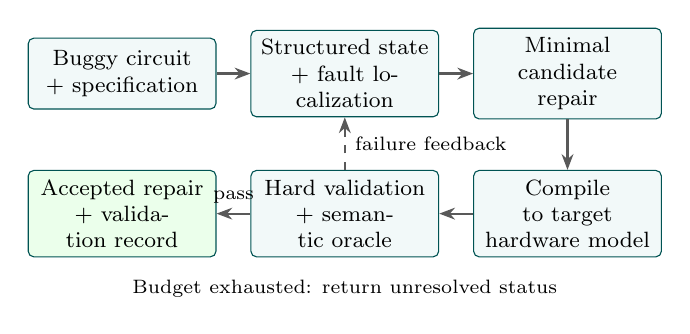
\begin{tikzpicture}[
    box/.style={draw=teal!65!black, rounded corners=2pt, fill=teal!5,
      text width=2.15cm, minimum height=0.9cm, align=center, font=\footnotesize},
    link/.style={-{Stealth[length=2mm]}, thick, draw=black!65},
    node distance=0.48cm and 0.43cm]
\node[box] (input) {Buggy circuit\\+ specification};
\node[box, right=of input] (state) {Structured state\\+ fault localization};
\node[box, right=of state] (repair) {Minimal candidate\\repair};
\node[box, below=0.64cm of repair] (compile) {Compile to target\\hardware model};
\node[box, left=of compile] (validate) {Hard validation\\+ semantic oracle};
\node[box, left=of validate, fill=green!8] (accept) {Accepted repair\\+ validation record};
\draw[link] (input) -- (state);
\draw[link] (state) -- (repair);
\draw[link] (repair) -- (compile);
\draw[link] (compile) -- (validate);
\draw[link] (validate) -- node[above, font=\scriptsize]{pass} (accept);
\draw[link, dashed] (validate) -- node[right, font=\scriptsize]{failure feedback} (state);
\node[below=0.16cm of validate, font=\scriptsize, align=center]
  {Budget exhausted: return unresolved status};
\end{tikzpicture}}
\caption{Proposed repair architecture. Dashed feedback carries failed-check diagnostics to the next decision step. Only a passing candidate is returned as an accepted repair.}
\label{fig:architecture}
\end{figure}

Localization prioritizes evidence from parsing failures, illegal operands, and behavior mismatches. Candidate generation then targets a limited region rather than rewriting an entire circuit without a reason. This design makes each change easier to inspect and helps distinguish a necessary routing transformation from an unrelated modification. The framework does not assume that the smallest textual patch is always the cheapest physical implementation.

\subsection{Constraint-Aware Candidate Selection}
The candidate-ranking objective is
\begin{equation}
 J(C)=\alpha S(C)+\beta P(C)+\gamma H(C)-\delta R(C),
\label{eq:objective}
\end{equation}
where $S$ measures semantic agreement, $P$ summarizes physical suitability, $H$ measures hardware compatibility, and $R$ penalizes unnecessary edits. Here $H(C)$ is a score, distinct from the history $H_t$. The weights are design parameters; numerical values are not available in the reported record. A reproducible instantiation must state the score scales and weights before evaluation.

Equation~\ref{eq:objective} cannot override the hard acceptance predicate. If several candidates satisfy Eq.~\ref{eq:accept}, the score can rank them; a high score never compensates for a failed semantic or physical check. This separation avoids an undesirable tradeoff in which an invalid circuit is selected merely because it uses fewer gates. Minimal editing is a preference within a valid solution set rather than permission to weaken correctness.

\subsection{Validation and Feedback Protocol}
Validation proceeds from inexpensive checks toward more demanding ones. Parsing and type checks reject malformed code. Structural checks examine register bounds, operand distinctness where required, and gate arity. Compilation maps a structurally valid candidate to the target. Semantic checks then account for the compiled circuit's output mapping, and physical checks assess the target-model requirements. Early rejection avoids running costly behavior checks on an unusable candidate.

\begin{figure}[t]
\begin{minipage}{\columnwidth}
\hrule\smallskip
\textbf{Algorithm 1:} Specification of the bounded repair loop
\smallskip\hrule\smallskip
\footnotesize
\begin{algorithmic}[1]
\REQUIRE Buggy circuit $C_{\mathrm{bug}}$, oracle $\mathcal O$, target $\mathcal B$, budget $K$
\STATE Initialize state $s$ with $C_{\mathrm{bug}}$ and diagnostics
\FOR{$t=1$ to $K$}
  \STATE Localize a fault using $s$ and propose candidate $C$
  \STATE Check syntax and structure of $C$
  \IF{the preliminary checks pass}
    \STATE Compile $C$ to $\widetilde C$ for $\mathcal B$
    \STATE Evaluate semantic and physical requirements
    \IF{$A(C;\mathcal O,\mathcal B)$ is true}
      \STATE \textbf{return} $\widetilde C$ and validation record
    \ENDIF
  \ENDIF
  \STATE Update $s$ with the candidate and failure diagnostics
\ENDFOR
\STATE \textbf{return} unresolved status and repair history
\end{algorithmic}
\smallskip\hrule
\end{minipage}
\end{figure}

Algorithm~1 gives a serial candidate loop. An implementation that generates multiple candidates per attempt should disclose that multiplicity and charge the associated tool calls to the evaluation budget. Failure records should identify the failing stage, relevant instruction or qubit, and any measured deviation. Budget exhaustion is an unresolved outcome, not an implicit acceptance of the last patch. Explicit unresolved status is especially important when an oracle is incomplete or a validator cannot finish.

\subsection{Illustrative Circuit Repair}
Figure~\ref{fig:circuit} illustrates gate-redundancy repair in a two-qubit circuit. Starting from $|00\rangle$, a Hadamard gate and controlled-NOT prepare the ideal Bell state
\begin{equation}
 |\Phi^+\rangle=(|00\rangle+|11\rangle)/\sqrt{2}.
\end{equation}
Two consecutive $X$ gates on the second qubit multiply to the identity, so removing the pair preserves the ideal transformation. The example demonstrates a local algebraic justification for a patch. It does not establish a measured fidelity gain: any such claim would require a specified noise model and execution data.

\begin{figure}[t]
\centering
\resizebox{\columnwidth}{!}{%
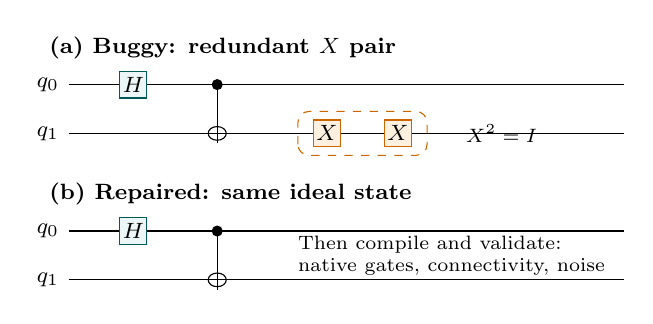
\begin{tikzpicture}[x=0.82cm,y=0.62cm, font=\footnotesize,
    gate/.style={draw=teal!70!black, fill=teal!7, minimum size=0.34cm, inner sep=1pt}]
\node[anchor=west, font=\footnotesize\bfseries] at (-0.45,0.75) {(a) Buggy: redundant $X$ pair};
\draw (0,0) -- (8.6,0);
\draw (0,-1) -- (8.6,-1);
\node[left] at (0,0) {$q_0$};
\node[left] at (0,-1) {$q_1$};
\node[gate] at (1,0) {$H$};
\draw (2.3,0) -- (2.3,-1);
\fill (2.3,0) circle (2pt);
\draw (2.3,-1) circle (0.14);
\draw (2.3,-1.2) -- (2.3,-0.8);
\node[gate, draw=orange!80!black, fill=orange!12] at (4,-1) {$X$};
\node[gate, draw=orange!80!black, fill=orange!12] at (5.1,-1) {$X$};
\draw[orange!80!black, dashed, rounded corners] (3.55,-1.45) rectangle (5.55,-0.55);
\node[anchor=west, font=\scriptsize] at (6,-1) {$X^2=I$};
\node[anchor=west, font=\footnotesize\bfseries] at (-0.45,-2.25) {(b) Repaired: same ideal state};
\draw (0,-3) -- (8.6,-3);
\draw (0,-4) -- (8.6,-4);
\node[left] at (0,-3) {$q_0$};
\node[left] at (0,-4) {$q_1$};
\node[gate] at (1,-3) {$H$};
\draw (2.3,-3) -- (2.3,-4);
\fill (2.3,-3) circle (2pt);
\draw (2.3,-4) circle (0.14);
\draw (2.3,-4.2) -- (2.3,-3.8);
\node[anchor=west, font=\scriptsize, align=left] at (3.4,-3.5)
  {Then compile and validate:\\native gates, connectivity, noise};
\end{tikzpicture}}
\caption{Illustrative redundancy repair, not a sampled benchmark result. Removing the highlighted $X$ pair preserves ideal semantics. The repaired logical circuit still requires target compilation and validation.}
\label{fig:circuit}
\end{figure}

The same principle also explains why local gate reduction is not the final objective. After removing a redundant pair, the remaining controlled operation may still require decomposition or routing. The agent must therefore validate the compiled candidate rather than infer hardware suitability from the simpler logical diagram alone.

\section{Experimental Setup and Metrics}
\subsection{Benchmark and Comparison Scope}
The reported benchmark contains 1,000 buggy circuits, equally distributed across five categories with 200 instances each. PyZX, QBugLM, and the proposed agent are each evaluated on all circuits, yielding 3,000 system-level evaluations. This count is not the number of candidate executions or independent experimental repetitions. The hardware model is IBM FakeSherbrooke; no live-hardware measurements are reported here.

The available material consists of aggregate tables rather than per-circuit traces. It does not specify the language-model version, prompts, sampling settings, compiler version, random seeds, circuit-size distribution, or noise thresholds. We therefore retain the reported values without filling these gaps with assumed settings. The framework description specifies the intended design, while the tables summarize the supplied evaluation record.

\subsection{Repair Success and Validity}
Let $y_{i,t}=1$ when attempt $t$ correctly repairs circuit $i$ under the benchmark oracle, and zero otherwise. The empirical cumulative success measure is
\begin{equation}
 \operatorname{Pass@}k=\frac{100}{N}\sum_{i=1}^{N}
 \ind\!\left[\max_{1\leq t\leq k}y_{i,t}=1\right],
 \quad N=1000.
\end{equation}
This definition means success within $k$ attempts, rather than a combinatorial estimator based on a larger sampled candidate pool. Physics validity is the percentage satisfying the hardware-grounded validation suite. It is reported separately and should not be substituted for full repair success.

Let $I_i$ denote the number of attempts used on circuit $i$. Mean iterations summarize the search effort but exclude differences in token use, simulation cost, and compilation time. For a structural resource $M$, the reduction convention is
\begin{equation}
 \Delta M_i=100\frac{M(C_{\mathrm{bug},i})-M(C_{\mathrm{repair},i})}
 {M(C_{\mathrm{bug},i})}.
\end{equation}
This expression assumes a nonzero input resource count. A complete protocol must state how empty circuits, failed repairs, and pre- versus post-compilation counts are handled. Negative reductions mean resource increases relative to the measured input, not negative gate counts.

\subsection{Uncertainty and Statistical Reporting}
The source tables report means and standard deviations. For a per-case binary metric encoded as 0 or 100, the standard deviation is approximately
\begin{equation}
 \sigma_{\mathrm{binary}}=100\sqrt{p(1-p)},
\end{equation}
where $p$ is the corresponding success fraction. Thus, a large standard deviation near a mid-range success rate does not, by itself, show instability across experimental runs or heterogeneous circuit families. These deviations are not confidence intervals. Without the raw observations, the sampling unit, pairing, and uncertainty calculations cannot be independently reconstructed.

\section{Results and Analysis}
\subsection{Overall Repair Performance}
Table~\ref{tab:overall} retains the primary reported results, and Fig.~\ref{fig:performance} compares their means. The proposed agent achieves 77.5\% Pass@1, exceeding QBugLM by 39.4 percentage points and PyZX by 72.5 points. Its Pass@3 is 99.1\%, corresponding to improvements of 61.0 and 94.1 points over the respective supplied baseline rows. These are absolute percentage-point differences, not relative percentage gains.

\begin{table}[t]
\caption{Reported correctness metrics (\%, mean $\pm$ SD). The SD describes the supplied outcomes, not a confidence interval.}
\label{tab:overall}
\centering\footnotesize
\begin{tabular}{@{}lrrr@{}}
\toprule
System & Pass@1 & Pass@3 & Physics validity\\
\midrule
PyZX & $5.0\pm21.8$ & $5.0\pm21.8$ & $15.5\pm36.2$\\
QBugLM & $38.1\pm48.6$ & $38.1\pm48.6$ & $69.6\pm46.0$\\
Ours & $77.5\pm41.8$ & $99.1\pm9.4$ & $99.2\pm8.9$\\
\bottomrule
\end{tabular}
\end{table}

\begin{figure}[t]
\centering
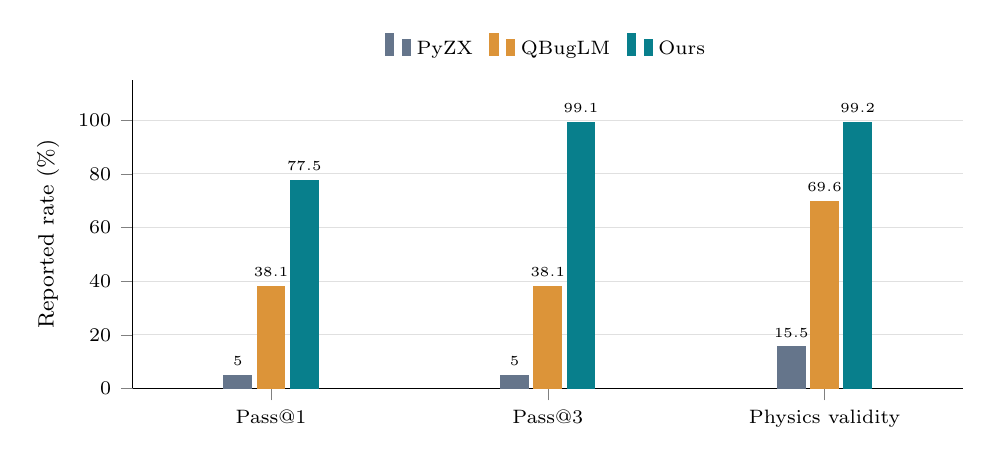
\begin{tikzpicture}
\begin{axis}[paperaxis, width=\columnwidth, height=5.5cm,
    ybar=2pt, bar width=10pt, ymin=0, ymax=115,
    xmin=-0.5, xmax=2.5, xtick={0,1,2},
    xticklabels={Pass@1,Pass@3,Physics validity},
    ytick={0,20,40,60,80,100}, ylabel={Reported rate (\%)},
    nodes near coords, every node near coord/.append style={font=\tiny},
    legend style={at={(0.5,1.03)}, anchor=south, legend columns=3,
      draw=none, font=\scriptsize, /tikz/every even column/.append style={column sep=4pt}}]
\addplot[fill=baseline, draw=baseline] coordinates {(0,5.0) (1,5.0) (2,15.5)};
\addplot[fill=language, draw=language] coordinates {(0,38.1) (1,38.1) (2,69.6)};
\addplot[fill=proposed, draw=proposed] coordinates {(0,77.5) (1,99.1) (2,99.2)};
\legend{PyZX,QBugLM,Ours}
\end{axis}
\end{tikzpicture}
\caption{Primary success and validity rates from Table~\ref{tab:overall}. Labels show reported percentages; no confidence intervals or new experimental observations are implied.}
\label{fig:performance}
\end{figure}

Physics validity reaches 99.2\%, compared with 69.6\% for QBugLM and 15.5\% for PyZX. Its 0.1-point difference from Pass@3 illustrates why the metrics should not be treated as interchangeable. The aggregate tables do not identify the overlap between semantic failures and physical failures, so they cannot establish which individual circuits account for that difference.

\subsection{Iteration and Recovery}
The proposed agent improves from 77.5\% on the first attempt to 99.1\% within three attempts, a gain of 21.6 points. If both percentages use the same 1,000 cases, these values correspond to 775 and 991 repaired circuits. Thus, 216 of the 225 initially unsuccessful cases are recovered, or 96.0\% of first-attempt failures. This is an arithmetic interpretation of the reported cumulative rates, not a newly measured recovery experiment.

No Pass@2 value or per-attempt trace is provided, so an intermediate learning curve cannot be reconstructed. The mean of 1.31 attempts also does not identify the full attempt distribution. For both baselines, Pass@1 equals Pass@3 and the reported mean is exactly one attempt. Consequently, the observed multi-attempt advantage combines an architectural comparison with unequal retry use. A budget-matched retry experiment is necessary to isolate the effect of physical feedback.

\subsection{Category-Level Coverage}
Figure~\ref{fig:coverage} visualizes the supplied violation-coverage table. The proposed agent reports 100\% for physics, semantics, and gate redundancy, 98\% for structure, and 97.5\% for syntax. Its gains over QBugLM are respectively 100, 73, 0, 82.5, and 49.5 percentage points. QBugLM also reaches 100\% on redundancy, while PyZX reaches 25\% in that category.

\begin{figure}[t]
\centering
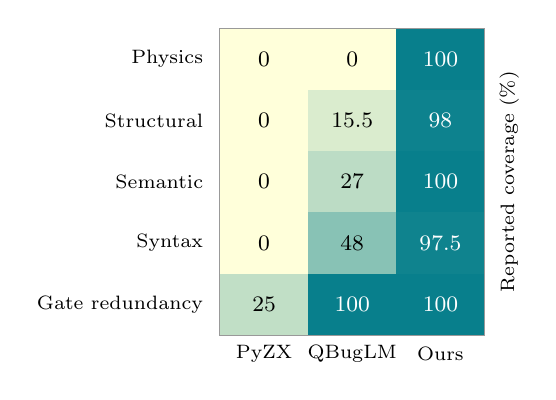
\begin{tikzpicture}[x=1.12cm,y=0.78cm, font=\footnotesize]
\foreach \category/\row in {Physics/0,Structural/1,Semantic/2,Syntax/3,Gate redundancy/4}{
  \node[anchor=east, font=\scriptsize] at (-0.08,-\row-0.5) {\category};
}
\foreach \system/\column in {PyZX/0,QBugLM/1,Ours/2}{
  \node[font=\scriptsize] at (\column+0.5,-5.3) {\system};
}
\foreach \column/\row/\value in {
    0/0/0,1/0/0,2/0/100,
    0/1/0,1/1/15.5,2/1/98,
    0/2/0,1/2/27,2/2/100,
    0/3/0,1/3/48,2/3/97.5,
    0/4/25,1/4/100,2/4/100}{
  \pgfmathtruncatemacro{\shade}{\value}
  \fill[proposed!\shade!heatlow] (\column,-\row) rectangle ++(1,-1);
  \ifnum\shade>64
    \node[text=white] at (\column+0.5,-\row-0.5) {\value};
  \else
    \node[text=black] at (\column+0.5,-\row-0.5) {\value};
  \fi
}
\draw[black!40] (0,0) rectangle (3,-5);
\node[rotate=90, font=\scriptsize] at (3.28,-2.5) {Reported coverage (\%)};
\end{tikzpicture}
\caption{Reported category-level violation coverage (\%). The coverage definition is not sufficiently specified to equate these cells with per-category Pass@3 or overall physics validity.}
\label{fig:coverage}
\end{figure}

These cells must be interpreted cautiously. Averaging the five equally weighted category values yields 99.1\% for the proposed method, but only 38.1\% for QBugLM and 5.0\% for PyZX. Those numbers align with the reported Pass@3 values, not with the overall physics-validity column. This numerical alignment does not prove that the quantities share a definition; it instead motivates clarifying the category table's numerator, denominator, and success criterion before treating it as a breakdown of physical validity.

\subsection{Structural Overhead and Repair Cost}
Table~\ref{tab:cost} and Fig.~\ref{fig:overhead} present the efficiency measures. The proposed method uses 1.31 mean iterations compared with 1.00 for the two baselines. Its mean gate-count and depth reductions are $-9.5\%$ and $-10.0\%$, indicating increases on average. The method therefore has the strongest reported correctness scores, but not the best structural reduction.

\begin{table}[t]
\caption{Reported repair effort and structural changes (mean $\pm$ SD). Reductions are percentages; iterations are counts.}
\label{tab:cost}
\centering\footnotesize
\begin{tabular}{@{}lrrr@{}}
\toprule
System & Iterations & Gate reduction & Depth reduction\\
\midrule
PyZX & $1.00\pm0.00$ & $-8.4\pm13.8$ & $-6.3\pm11.0$\\
QBugLM & $1.00\pm0.00$ & $-7.8\pm15.6$ & $-8.1\pm16.0$\\
Ours & $1.31\pm0.62$ & $-9.5\pm16.8$ & $-10.0\pm17.2$\\
\bottomrule
\end{tabular}
\end{table}

\begin{figure}[t]
\centering
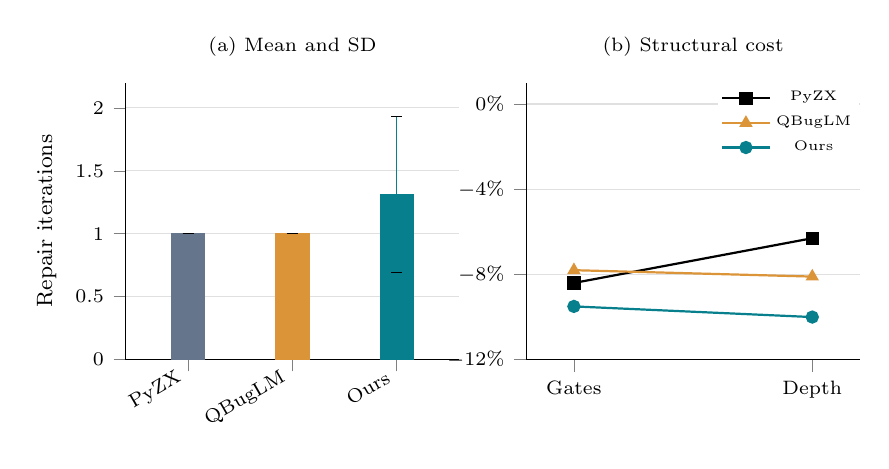
\begin{tikzpicture}
\begin{axis}[paperaxis, name=iterations, width=0.48\columnwidth, height=5.1cm,
    title={(a) Mean and SD}, title style={font=\scriptsize},
    ybar, bar width=12pt, ymin=0, ymax=2.2, xmin=-0.6, xmax=2.6,
    xtick={0,1,2}, xticklabels={PyZX,QBugLM,Ours},
    x tick label style={rotate=30,anchor=east,font=\scriptsize},
    ylabel={Repair iterations},
    error bars/y dir=both, error bars/y explicit]
\addplot[fill=baseline, draw=baseline, bar shift=0pt] coordinates {(0,1) +- (0,0)};
\addplot[fill=language, draw=language, bar shift=0pt] coordinates {(1,1) +- (0,0)};
\addplot[fill=proposed, draw=proposed, bar shift=0pt] coordinates {(2,1.31) +- (0,0.62)};
\end{axis}
\begin{axis}[paperaxis, at={(iterations.east)}, anchor=west, xshift=0.85cm,
    width=0.48\columnwidth, height=5.1cm,
    title={(b) Structural cost}, title style={font=\scriptsize},
    ymin=-12, ymax=1, xmin=-0.2, xmax=1.2,
    xtick={0,1}, xticklabels={Gates,Depth},
    ytick={-12,-8,-4,0}, yticklabel={\pgfmathprintnumber{\tick}\%},
    legend style={at={(1,1)}, anchor=north east, draw=none,
      font=\tiny, inner sep=1pt}]
\addplot[baseline, mark=square*, thick] coordinates {(0,-8.4) (1,-6.3)};
\addplot[language, mark=triangle*, thick] coordinates {(0,-7.8) (1,-8.1)};
\addplot[proposed, mark=*, thick] coordinates {(0,-9.5) (1,-10.0)};
\legend{PyZX,QBugLM,Ours}
\end{axis}
\end{tikzpicture}
\caption{Repair effort and structural overhead. (a) Mean iterations with reported SD. (b) Mean gate-count and depth reductions; negative values indicate increases. Connecting lines distinguish systems, not a temporal trend.}
\label{fig:overhead}
\end{figure}

Routing, decomposition, and restoring missing operations are plausible reasons for such increases, but the aggregate data do not attribute overhead to any specific transformation. Nor do they establish that every additional gate is necessary. A useful follow-up would separate logical repair cost from compilation cost and report resource changes on a common subset of successfully repaired circuits. Without that conditioning, a system that leaves many cases unresolved may appear structurally cheaper for the wrong reason.

\subsection{Reported Pairwise Statistics}
Table~\ref{tab:stats} reproduces the supplied $W$, $p$, and $d$ values. They have not been recomputed from paired circuit outcomes. The record does not specify the exact test variant, treatment of ties and zero differences, definition of $d$, or correction for multiple comparisons. We omit a categorical effect-size label because its interpretation depends on the effect-size definition and chosen convention.

\begin{table}[t]
\caption{Pairwise statistics retained from the supplied results. Test details and effect-size definitions require verification against the underlying paired records.}
\label{tab:stats}
\centering\scriptsize
\begin{tabular}{@{}llrrr@{}}
\toprule
Comparison & Metric & $W$ & $p$ & $d$\\
\midrule
Ours/QBugLM & Pass@1 & 1603.0 & $8.11\times10^{-87}$ & .799\\
Ours/QBugLM & Pass@3 & 0 & $1.12\times10^{-134}$ & 1.250\\
Ours/QBugLM & Physics & 2548.5 & $4.68\times10^{-65}$ & .639\\
Ours/PyZX & Pass@1 & 0 & $1.10\times10^{-159}$ & 1.623\\
Ours/PyZX & Pass@3 & 0 & $1.20\times10^{-206}$ & 3.992\\
Ours/PyZX & Physics & 0 & $4.87\times10^{-184}$ & 2.265\\
\bottomrule
\end{tabular}
\end{table}

The descriptive rate differences remain directly readable from Table~\ref{tab:overall}, but extremely small reported $p$-values do not resolve uncertainty about configuration fairness or oracle quality. Per-case outcomes and the analysis script are required for an independent statistical audit. They would also allow the comparison to account for circuits derived from the same underlying program, if such clustering exists.

\section{Discussion and Threats to Validity}
\subsection{What the Evidence Supports}
The reported configuration achieves high cumulative repair success and high model-based physics validity. The large first-to-third-attempt improvement is consistent with useful feedback-driven search. However, the summaries alone do not establish a causal contribution from each component. Physical validation, language-model choice, prompts, candidate multiplicity, and additional retries can all affect the outcome. The central architectural recommendation is therefore to expose and enforce independent checks, rather than to claim that a particular component has been isolated experimentally.

The circuit example also highlights the relationship between repair and optimization. Redundancy removal is a valid local transformation, but semantic fault repair may need to insert a missing operation. Resource reduction should be a secondary objective after restoring the specification. At the same time, validity should not become a blanket justification for avoidable overhead; accepted candidates can still be compared for cost under the same target model.

\subsection{Internal and Construct Validity}
The semantic oracle is a central source of risk. A small collection of output tests can miss faults, while an incorrect reference can reward the wrong behavior. The physical-validity label has a similar dependence on the breadth of its checks. Native-gate acceptance, successful routing, and a noise-aware performance threshold measure different properties and should be logged separately. Aggregate validity rates obscure which checks are responsible for rejection.

Baseline scope also matters. PyZX is fundamentally a transformation tool, and QBugLM supports richer workflows than the one-attempt summary implies. The present comparison therefore cannot establish universal superiority over either system. The absence of model settings and equalized candidate budgets further limits attribution. These concerns affect the interpretation of the existing numbers; they are not resolved by drawing additional plots from the same aggregates.

\subsection{External Validity and Reproducibility}
\balance
An equal five-class benchmark is convenient for coverage but need not reflect the prevalence of bugs in practical projects. Generalization to human-authored faults, larger circuits, different programming styles, and additional devices remains unmeasured. FakeSherbrooke provides a hardware-model setting, not evidence that the repair loop handles changing calibration on a live backend. Calibration drift and scheduling constraints should be treated as future evaluation targets rather than demonstrated capabilities.

A reproducibility package should include circuit identifiers, bug-injection rules, trusted reference behavior, all attempted patches, and stage-level validator outputs. It should also record the model and prompt configuration, compilation settings, target snapshot, execution seeds, and sampling budget. Those records would make it possible to distinguish repair failures from validator failures and to regenerate the statistical analysis. The visualizations in this paper can be reproduced from the supplied aggregates, but they cannot substitute for those experimental artifacts.

\subsection{Priority Follow-Up Experiments}
The most informative ablation would hold the model, prompts, and three-attempt budget fixed while changing only the availability of physical-validation feedback. A second comparison should separate the benefit of accepting only physically valid repairs from the benefit of explaining physical failures to the generator. An oracle-only rejection rule and a diagnostic-feedback rule may produce different search behavior even when they use the same acceptance predicate.

Additional experiments should measure wall-clock time, tool calls, and token usage alongside repair iterations. Testing across target models and calibration snapshots would assess whether the accepted repairs remain robust when the physical assumptions change. No ablation, latency, or cross-device measurements are claimed here because the corresponding experimental records are not available.

\section{Conclusion}
This paper presents a physics-constrained architecture for automated quantum-circuit debugging and repair. Structured state, minimal edits, compilation, and independent validation form a bounded feedback loop with explicit unresolved outcomes. The supplied 1,000-circuit benchmark reports 77.5\% Pass@1, 99.1\% Pass@3, and 99.2\% physics validity for the proposed configuration, at the cost of additional iterations and structural overhead. These descriptive results motivate treating physical executability as a hard acceptance requirement. Matched-budget baselines, documented oracles, per-circuit traces, and cross-device experiments are needed to establish the individual sources and practical scope of the observed gains.

\section*{Acknowledgment}
The author thanks the open-source quantum software community and the researchers whose work informed the benchmark design and related-work analysis.

\begin{thebibliography}{6}
\bibitem{guo2024repairing}
X. Guo, J. Zhao, and P. Zhao, ``On repairing quantum programs using ChatGPT,''
in \emph{Proc. IEEE/ACM 5th Int. Workshop on Quantum Software Engineering (Q-SE)},
2024, pp. 9--16.

\bibitem{pham2026qbuglm}
A. B. B. Pham, H. T. Nguyen, and M. Usman, ``QBugLM: An agentic benchmarking
framework for LLM-based quantum software debugging,''
\emph{arXiv preprint arXiv:2606.07314}, 2026.

\bibitem{duncan2020graph}
R. Duncan, A. Kissinger, S. Perdrix, and J. van de Wetering,
``Graph-theoretic simplification of quantum circuits with the ZX-calculus,''
\emph{Quantum}, vol. 4, p. 279, 2020.

\bibitem{quarl2024}
Z. Li, J. Peng, Y. Mei, S. Lin, Y. Wu, O. Padon, and Z. Jia,
``Quarl: A learning-based quantum circuit optimizer,''
\emph{Proc. ACM Program. Lang.}, vol. 8, no. OOPSLA1, 2024.

\bibitem{ernst2025physical}
J. O. Ernst, A. Chatterjee, T. Franzmeyer, and A. Kuhn,
``Reinforcement learning for quantum control under physical constraints,''
in \emph{Proc. 42nd Int. Conf. Machine Learning},
ser. Proceedings of Machine Learning Research, vol. 267, 2025.

\bibitem{ibmnoise}
IBM Quantum, ``Build noise models,'' IBM Quantum Documentation,
accessed: Sep. 13, 2026. [Online]. Available:
\url{https://quantum.cloud.ibm.com/docs/en/guides/build-noise-models}
\end{thebibliography}
\end{document}
